\documentclass{article}
\usepackage{neurips_2026}
\usepackage[utf8]{inputenc}
\usepackage[T1]{fontenc}
\usepackage{hyperref}
\usepackage{url}
\usepackage{booktabs}
\usepackage{amsfonts,amsmath,amssymb}
\usepackage{nicefrac}
\usepackage{microtype}
\usepackage{xcolor}
\usepackage{graphicx}
\usepackage{multirow}

\newcommand{\phat}{\hat\phi}
\newcommand{\E}{\mathbb{E}}

\title{When Is a Single SHAP Run Enough? Repeat-Run Reliability of Sampled Shapley Attributions on Tabular Models}

\author{Anonymous Authors}

\begin{document}
\maketitle

\begin{abstract}
SHAP explanations are usually produced by a randomized estimator, run once per instance under a fixed compute budget, and then read as ``the reason'' for a prediction. We ask when that single run can be trusted. Exact Shapley values are available as ground truth for 8--20 players if all $2^d$ coalitions are tabulated, so we can repeat each estimator 100 times at budgets of 64--8192 coalition evaluations on 1{,}536 explained instance--model pairs (5 public tabular datasets, logistic regression, MLP, random forest, XGBoost), and check against a real-library run on 4 of these datasets and a $d{=}262$ stress test. The answer depends on the claim and the budget. At a budget close to the \texttt{shap} default ($m{=}2048$), one run names the correct top-1 feature in 99.4\% of cases and the correct top-3 set in 98.4\% (cell-weighted means, $d\ge16$), but 6\% of instance--model pairs still fail a 90\%-repeatability criterion at $m{=}2048$ and 21\% at $m{=}256$; every failure at $m{=}2048$ is a near-tie ($3^{\rm rd}$ vs.\ $4^{\rm th}$ attribution within 2\% of $\|\phi\|_2$). Reliability collapses onto one curve, $\Phi(z)$, of an instance's gap-to-noise ratio $z$. $z$ can be estimated from the run itself with a sandwich standard error at no extra model calls: certifying runs with $z\ge2$ keeps 92\% of runs at $m{=}2048$ with 0.04\% top-3 errors, and has lower error than a cost-matched two-run agreement check at equal coverage for $m\le512$. Coalition-sampling noise is much smaller than the variation from retraining the model or redrawing a 100-row background; at fixed model-call budget, background rows are the better use of compute for $d\le10$. Finally, \texttt{shap}'s default \texttt{l1\_reg} makes errors 10$\times$ larger at $d{=}20$ and fails at $d{=}262$.
\end{abstract}

\section{Introduction}
Shapley-value attributions \citep{lundberg2017} are used to justify individual predictions in credit, health and other high-stakes settings. For anything other than trees or linear models, they are estimated by sampling coalitions of features, and the quality of the estimate is set by a compute budget: every coalition costs one pass of the model over the whole background sample. The common practice is to run the explainer once per instance and report the resulting attribution vector. Whether this is sufficient has two possible failure modes. The estimator may be noisy, so that a second run would name different features; and the noise, or the budget, may be unimportant next to other unavoidable sources of variation in the explanation, so that worrying about it is wasted effort. Both are empirical questions, and which one holds depends on the \emph{claim} made (``feature $j$ matters most'', ``these three features'', ``feature $j$ contributes $+0.07$''), the budget, the model, and the instance.

We study the question with a design that makes it checkable. For $d\le20$ players we tabulate the value function on all $2^d$ coalitions, so that (i) the exact Shapley values are known for the same game the estimators target, and (ii) running an estimator reduces to a table look-up that returns exactly what a run with real model calls would return, which lets us repeat each run 100 times at nine budgets. We validate this against the \texttt{shap} library with real model calls. Our contributions are:
\begin{itemize}\setlength\itemsep{0pt}
\item \textbf{A claim-level reliability protocol} with exact ground truth, repeat runs at explicit budgets, several agreement measures (top-1, top-3 set, RBO \citep{webber2010}, Nogueira stability \citep{nogueira2018}) and an instance-level criterion, with cluster-bootstrap uncertainty (\S\ref{sec:method}).
\item \textbf{Empirical answers} over 5 datasets $\times$ 4 models $\times$ 3 estimators (\S\ref{sec:headline}--\ref{sec:est}): single runs are adequate for coarse claims at moderate budgets, not for finer claims at low budgets or near-ties, and the reliability of the top-3 claim is a single function of one noise-to-gap statistic.
\item \textbf{A single-run certificate} from a within-run standard error that costs no extra model calls, evaluated against exact truth and against a cost-matched repeat check (\S\ref{sec:cert}).
\item \textbf{Yardsticks}: the estimator's disagreement is compared to that caused by retraining the model, by redrawing the background, and by the defaults of the \texttt{shap} library (\S\ref{sec:yard}, \ref{sec:highd}).
\end{itemize}
We report negative and null findings as they came out (e.g.\ the leverage-score sampler of \citet{musco2024} gives no meaningful gain over Kernel SHAP at our budgets; the high-dimensional stress test is easier than anticipated for our estimators, though not for the library default).

\section{Related work}
\textbf{Shapley estimators.} Kernel SHAP \citep{lundberg2017} casts Shapley estimation as constrained weighted regression over sampled coalitions; permutation/Monte-Carlo sampling goes back to \citet{strumbelj2014}; TreeSHAP \citep{lundberg2020} is exact and deterministic for trees. \citet{covert2021} analyze Kernel SHAP, propose an unbiased variant, variance reduction, and use bootstrap-type estimates for convergence detection and uncertainty; \citet{mitchell2022} improve permutation sampling; \citet{musco2024} propose Leverage SHAP with provable guarantees; \citet{chen2023} survey the algorithms. These works measure estimator error on small numbers of models or instances; we instead ask what that error means for explanation \emph{claims} across many instances and models, and what a practitioner can do within a single run. We adopt the within-run uncertainty idea of \citet{covert2021} and test it (in a sandwich-variance form for the paired, partially enumerated sampler used in practice) as a claim-level certificate.

\textbf{Variability of explanations.} \citet{krishna2022} study disagreement between different explanation methods; \citet{yuan2022} study how the random background sample changes SHAP values and rankings for deep models on one clinical dataset; \citet{chen2020} discuss how the choice of expectation (interventional vs.\ observational) changes what Shapley values mean. We use the interventional game with a fixed background and then compare its estimator noise to the background and model effects. Our retraining comparison is in the spirit of predictive multiplicity \citep{marx2019}: equally accurate models need not give the same explanation.

\textbf{Measures.} We use stability of top-$k$ selection \citep{nogueira2018} and rank-biased overlap \citep{webber2010}, and the datasets of \citet{ding2021} and the UCI/OpenML repositories.

\section{Setting and methodology}\label{sec:method}
\paragraph{Target and budget.} For a model $f$ (probability of the positive class), an instance $x$ and a background sample $B=\{b_1..b_n\}$ ($n{=}100$ rows unless stated), the interventional value function is $v(S)=\frac1n\sum_r f(x_S,b_{r,\bar S})$ over $d$ players (original features; one-hot columns of a categorical feature form one player). The Shapley values $\phi\in\mathbb{R}^d$ of $v$ are the \emph{target}; we call them exact. A \emph{single run} of an estimator with budget $m$ evaluates $m$ coalitions (excluding $\emptyset$ and the full set) and returns $\phat$; its cost is $m\cdot n$ model calls. Randomness is only in the coalitions (background fixed) unless stated.

\paragraph{Estimators.} \emph{Kernel SHAP}: our numba port of the sampling logic of \texttt{shap.KernelExplainer} (paired sampling of complements, complete enumeration of the cheapest size classes while the budget allows, size-proportional sampling of the rest with duplicate counting, constrained weighted least squares) without the L1 feature selection step. \emph{Leverage SHAP}: the same machinery, drawing coalition sizes uniformly (the leverage scores of the Shapley regression are $1/\binom{d}{|S|}$, which we verified numerically) with Horvitz--Thompson weights; this is our re-implementation of the idea in \citet{musco2024}, not their code. \emph{Permutation SHAP}: antithetic (forward and reversed) permutations, $2(d-1)$ coalitions per pair. Details are in Appendix~\ref{app:est}.

\paragraph{Ground truth and the table oracle.} For each instance we evaluate $v$ on all $2^d$ coalitions ($d\le20$), compute $\phi$ exactly, and implement every estimator as a look-up in this table. Since the estimators only access $v$ through the values on the coalitions they sample, this returns exactly what a run with real model calls would return. We verify the equivalence against the real \texttt{shap} library in \S\ref{sec:est}. Budgets are $m\in\{32,64,\dots,8192\}$; $m=32$ is below $2d$ for $d\ge16$, where the regression is under-determined and a run can be arbitrarily wrong (we report it in the data release but exclude it from all analyses; Permutation SHAP needs $m\ge2(d-1)$). A dataset with $2^d-2\le m$ is enumerated exactly. The \texttt{shap} default is $m=2d+2048$.

\paragraph{Data, models, instances.} Table~\ref{tab:setup} lists the datasets: Pima Diabetes (OpenML 37), Give Me Some Credit (OpenML 46929, 40k-row subsample), ACSIncome and ACSEmployment \citep{ding2021} (California, 2018, 40k-row subsample), and German Credit \citep{german}. Models: $\ell_2$ logistic regression, a 2-layer MLP, random forest \citep{breiman2001} and XGBoost \citep{chen2016xgb} (scikit-learn \citep{pedregosa2011}; hyper-parameters fixed a priori, Appendix~\ref{app:setup}). One model per (dataset, model type) on a stratified 70/30 split; instances are drawn uniformly from the test split (100 each for $d\le10$, 60 for $d{=}16$, 24 for $d{=}20$ where each instance costs $2^{20}\cdot100$ model calls to tabulate). For each (instance, estimator, $m$) we do 100 independent runs. A replicate with a second split and model seed is in Appendix~\ref{app:rep}.

\begin{table}[t]
\centering\small\setlength{\tabcolsep}{4pt}
\begin{tabular}{lrrrrrcccc}
\toprule
Dataset & $n$ & $n_{\rm train}$ & $d$ & $b_{\rm ref}$ & \#inst. & \multicolumn{4}{c}{test AUC}\\
\cmidrule(lr){7-10}
 & & & & & & LR & MLP & RF & XGB\\
\midrule
Pima Diabetes & 768 & 537 & 8 & 500 & 100 & 0.867 & 0.869 & 0.847 & 0.834\\
Give Me Some Credit & 40000 & 28000 & 10 & 1000 & 100 & 0.853 & 0.864 & 0.865 & 0.866\\
ACSIncome (CA 2018) & 40000 & 28000 & 10 & 1000 & 100 & 0.889 & 0.899 & 0.898 & 0.902\\
ACSEmployment (CA 2018) & 40000 & 28000 & 16 & 100 & 60 & 0.876 & 0.902 & 0.904 & 0.905\\
German Credit & 1000 & 700 & 20 & 100 & 24 & 0.798 & 0.778 & 0.802 & 0.785\\
\bottomrule
\end{tabular}
\caption{Datasets and models. $d$: players; $b_{\rm ref}$: size of the reference background sample used to tabulate $v$ (the main experiments use its first 100 rows); \#inst.: explained test instances per model.}\label{tab:setup}
\end{table}

\paragraph{Claims and reliability measures.} For each run we compare $\phat$ to $\phi$ on: relative $\ell_2$ error; \textbf{top-1} (is $\arg\max_j|\phat_j|$ the exact one); \textbf{top-3 set} (is the set of the three largest $|\phat_j|$ exactly the exact set); sign agreement on the exact top-3; Spearman correlation and RBO ($p{=}0.9$) of the $|\cdot|$-rankings. For repeatability we also compare 200 random pairs of independent runs (agreement of top-3 sets, RBO) and compute the Nogueira stability of top-3 selection over the 100 runs. The \textbf{instance-level criterion} is: a single run is \emph{reliable for a claim} on instance $x$ if the claim is correct in at least 90\% of runs; we report the fraction of instances that satisfy it (so a run-averaged success rate of 98\% can hide a 10\% minority of unreliable instances). The 0.9 level is a convention, not a standard; Fig.~\ref{fig:budget} and Appendix~\ref{app:more} show other views.

\paragraph{Statistics.} The unit of analysis is the explained instance. Results per (dataset, model) cell are means over instances; pooled numbers are equal-weight means over cells; 95\% intervals are percentile intervals from a cluster bootstrap that resamples instances within each cell (1000--2000 resamples). They quantify \emph{instance sampling} uncertainty and, via the 100 runs per instance, run-to-run noise; they do not include variation across independently trained models, which we address only by the small replicate and the retraining experiment. Intervals for rates near 0 (e.g.\ certified error) are bootstrap intervals over instance clusters and are approximate.

\paragraph{Single-run diagnostic.} For Kernel SHAP the sampled draws $j=1..N$ (a draw is a coalition and its complement) are iid, so the estimator $\phat=A^{-1}\sum_j g_j$ in the reduced $(d-1)$-parameter regression has a sandwich covariance $\hat V=A^{-1}\big[\tfrac{N}{N-1}\sum_j(g_j-\bar g)(g_j-\bar g)^\top\big]A^{-1}$ in which the enumerated part contributes no variance; for Permutation SHAP the standard error is the sample SD over permutation pairs divided by $\sqrt{\#\text{pairs}}$. Neither needs a model call beyond the run. For the top-3 claim, sort $|\phat|$ and define $z_3=(a_{(3)}-a_{(4)})/\sqrt{\widehat{\rm se}_{(3)}^2+\widehat{\rm se}_{(4)}^2}$, and the \emph{certificate} ``$z_3\ge c$''; the \emph{oracle} version $z$ uses the exact gap and the empirical SD of the 100 runs.

\section{Results}
\subsection{How reliable is one run? It depends on the claim and the budget}\label{sec:headline}
\begin{figure}[t]
\centering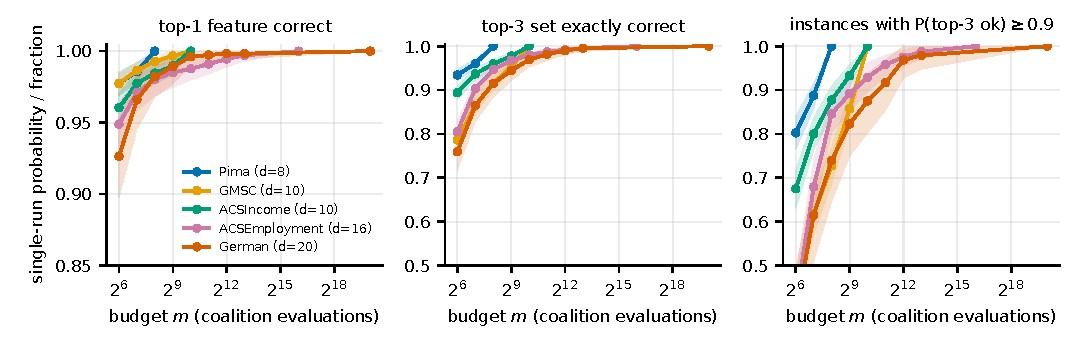
\includegraphics[width=\textwidth]{figs/fig_reliability_budget.pdf}
\caption{Single-run reliability of Kernel SHAP vs.\ budget for the five datasets (mean over 4 models; bands: 95\% cluster-bootstrap CI). The final point of each line is complete enumeration ($2^d-2$ evaluations), which is exact. Left: probability that the top-1 feature is correct; middle: that the top-3 set is correct; right: fraction of instances for which the top-3 claim is correct in $\ge$90\% of runs.}\label{fig:budget}
\end{figure}
Fig.~\ref{fig:budget} and Table~\ref{tab:rel} (Appendix) give the main picture. For the two datasets with $d\ge16$, pooled over the 8 (dataset, model) cells, a Kernel SHAP run at $m{=}2048$ (the default budget is $m{=}2d{+}2048$) names the exact top-1 feature in 99.4\% [99.0, 99.8] of runs and the exact top-3 set in 98.4\% [97.7, 99.1], with mean relative $\ell_2$ error 1.4\%. The top-3 claim is considerably weaker at lower budgets: 93.1\% [91.4, 94.6] at $m{=}256$ and 78.2\% [75.9, 80.8] at $m{=}64$ (top-1: 98.1\% and 93.8\%). The same budget yields different instance-level guarantees: the fraction of instances for which the top-3 claim meets the 90\% criterion is 93.8\% [90.7, 96.6] at $m{=}2048$, 79.3\% [74.6, 83.9] at $m{=}256$ and only 40.6\% [35.2, 46.5] at $m{=}64$. Among the 336 instance--model pairs with $d\ge16$ the median budget needed to meet the criterion is 128, the 90th percentile 1024, 5.4\% need more than 2048 and 1.5\% do not reach it by 8192. Run-to-run agreement of the top-3 set between two independent runs is 97.6\% [96.5, 98.5] at $m{=}2048$ and 90.1\% [88.0, 92.1] at $m{=}256$ (Nogueira stability 0.991 and 0.960; this measure is lenient here because only two or three features fluctuate between ranks).

Three qualifications matter. (i) For $d\le10$ the problem disappears at no larger cost than the default: complete enumeration needs $2^d-2\le1022$ evaluations, so noise can be eliminated; at the intermediate $m{=}256$ the top-3 claim is correct in 86--98\% of runs (GMSC) and 93--97\% (ACSIncome) depending on the model (Table~\ref{tab:rel}). (ii) Models differ, but not in a stable order: at $m{=}2048$ the fraction of reliable instances for $d\ge16$ is 96\% for LR, 96\% for RF, 94\% for XGBoost and 92\% for MLP (24--60 instances each), and a replicate with a different training split moves single cells by up to 16 points (Appendix~\ref{app:rep}), so we do not rank model families. (iii) Top-1 is much easier than top-3, and values are easier than ranks near ties: the pooled mean relative error is 4.8\% at $m{=}256$ and 0.6\% at $m{=}8192$.

\subsection{Where and why single runs fail}\label{sec:mech}
\begin{figure}[t]
\centering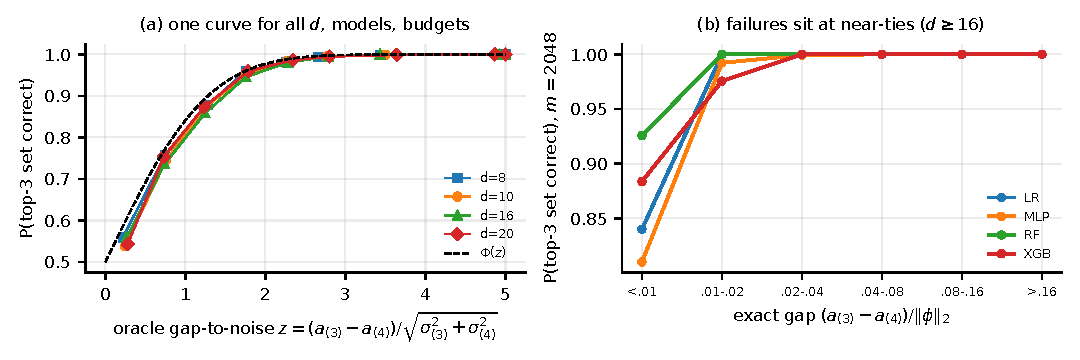
\includegraphics[width=\textwidth]{figs/fig_mechanism.pdf}
\caption{(a) Probability that a run recovers the exact top-3 set versus the oracle gap-to-noise ratio $z$ (binned; Kernel SHAP, all datasets, models and budgets $m\ge64$, bins with $\ge20$ instance--budget cells). The dashed line is the standard normal CDF. (b) At $m=2048$ and $d\ge16$ the failures are concentrated at near-ties of the exact attribution.}\label{fig:mech}
\end{figure}
A run errs on the top-3 set when noise reorders the 3rd and 4th largest attributions. If the estimate were Gaussian with the empirical SD $\sigma_j$ of each feature, the probability of preserving the order is $\approx\Phi(z)$ with $z=(a_{(3)}-a_{(4)})/\sqrt{\sigma_{(3)}^2+\sigma_{(4)}^2}$. Fig.~\ref{fig:mech}a shows this holds empirically: instance-by-budget cells from all five datasets, four models and all budgets lie close to $\Phi(z)$, regardless of $d$ (the observed probability is slightly below $\Phi(z)$ for $z\lesssim2$, e.g.\ 0.54 vs.\ 0.60 at $z\approx0.25$: the Gaussian two-feature approximation is mildly optimistic). The practical consequence is that the budget needed is set by the \emph{instance's} margin: the gap between the 3rd and 4th attribution relative to the run-to-run noise, where the noise shrinks faster than $m^{-1/2}$ (by a factor of about 1.5 per doubling of $m$ from $m{=}256$, since larger budgets also enumerate more size classes; Appendix Fig.~\ref{fig:sd}). At $m{=}2048$, 19.6\% of the $d\ge16$ instance--model pairs have a gap below $0.02\|\phi\|_2$, and \emph{all 18} pairs that fail the 90\% criterion are among them (Fig.~\ref{fig:mech}b): failures are near-ties. In those cases the claim ``these are the top three features'' is not well determined by the model's exact attribution either, so resolving them with more compute has little value. The noise level itself is tied to non-additivity: the share of the kernel-weighted variance of $v$ left unexplained by the additive game correlates with the relative run-to-run SD (Spearman 0.64 at $m{=}512$, $d\ge16$, 336 instance--model pairs; 0.70 within ACSEmployment, 0.51 within German).

\subsection{Estimators, and what the library default does}\label{sec:est}
\begin{table}[t]
\centering\small
\begin{tabular}{rcccccc}
\toprule
$m$ & \multicolumn{3}{c}{P(top-3 set correct), \%} & \multicolumn{3}{c}{median rel.\ $\ell_2$ error, \%}\\
\cmidrule(lr){2-4}\cmidrule(lr){5-7}
 & Kernel & Leverage & Perm. & Kernel & Leverage & Perm.\\
\midrule
64 & 78.2 & 79.4 & 81.1 & 12.25 & 11.40 & 7.57\\
128 & 88.4 & 88.8 & 87.5 & 6.54 & 6.22 & 5.08\\
256 & 93.1 & 93.5 & 90.9 & 4.00 & 3.73 & 3.58\\
512 & 95.6 & 96.2 & 94.0 & 2.60 & 2.43 & 2.44\\
2048 & 98.4 & 98.4 & 97.5 & 1.13 & 1.08 & 1.21\\
8192 & 99.5 & 99.6 & 99.2 & 0.47 & 0.46 & 0.61\\
\bottomrule
\end{tabular}
\caption{Estimators at equal budget, $d\ge16$ (336 instance--model pairs): pooled P(top-3 set correct) and median relative $\ell_2$ error. Paired differences in top-3 correctness (Leverage$-$Kernel, Permutation$-$Kernel, 95\% CI): $m{=}64$: +1.1 [0.4, 1.8] / +2.9 [1.9, 3.9] points; $m{=}256$: +0.4 [$-$0.1, 0.9] / $-$2.2 [$-$2.9, $-$1.4]; $m{=}2048$: $-$0.0 [$-$0.2, 0.1] / $-$0.9 [$-$1.3, $-$0.6].}\label{tab:est}
\end{table}
The three estimators are close (Table~\ref{tab:est}). Leverage SHAP differs from Kernel SHAP by at most +1.1 points of top-3 correctness at any budget (largest at $m{=}64$) and is indistinguishable from $m{=}2048$ on; Permutation SHAP is more accurate at the lowest budget but 0.4--2.2 points worse for top-3 from $m{=}128$ on. So the estimator is not the lever: the conclusions of \S\ref{sec:headline}--\ref{sec:mech} are not artefacts of Kernel SHAP.

\emph{Validation.} Running the real library (\texttt{shap} 0.51.0, XGBoost, 8 instances $\times$ 20 repeats per setting, real model calls) gives errors that match the table oracle at equal budget for Kernel SHAP with \texttt{l1\_reg=False}, e.g.\ median relative error on German 0.195/0.061/0.018 (library) vs.\ 0.217/0.067/0.020 (oracle) at $m{=}64/256/2088$ (Appendix Table~\ref{tab:lib}). The library's permutation explainer is somewhat worse than ours on ACSEmployment at $m{=}64$ (0.090 vs.\ 0.053; 8 instances) and similar elsewhere. \emph{The default matters.} The library's default is \texttt{l1\_reg="num\_features(10)"}, which keeps at most 10 features. For $d>10$ its error stops decreasing with the budget: German, default budget: 0.210 median relative error vs.\ 0.018 without it (top-3 set 98.8\% vs.\ 100\%); ACSEmployment: 0.031 vs.\ 0.012. This is a property of that default in that version, not of Kernel SHAP; it is invisible if one only repeats runs, since the error is a bias.

\subsection{Certifying a single run from itself}\label{sec:cert}
\begin{figure}[t]
\centering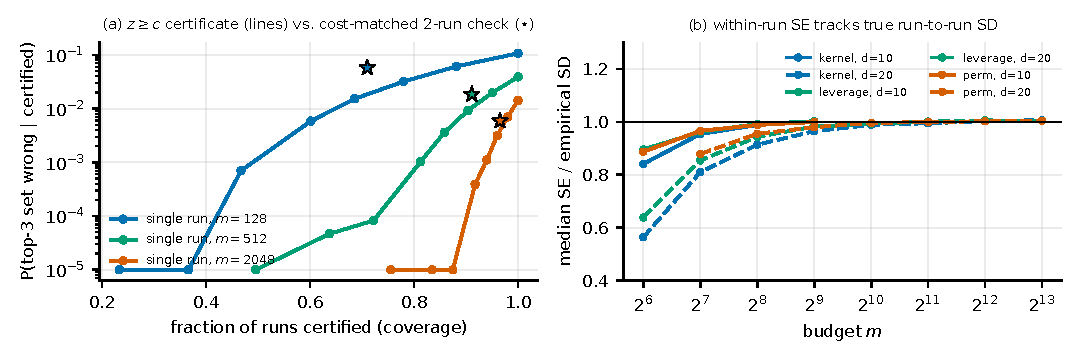
\includegraphics[width=\textwidth]{figs/fig_certificate.pdf}
\caption{(a) Error of the top-3 set among certified runs vs.\ certified fraction, as the threshold $c$ in ``$z_3\ge c$'' varies (lines; $d\ge16$ datasets, Kernel SHAP), and the cost-matched alternative of running twice at $m/2$ and certifying when the two top-3 sets agree (stars, error of the pooled estimate). (b) Ratio of the within-run standard error to the empirical SD across runs.}\label{fig:cert}
\end{figure}
\begin{table}[t]
\centering\scriptsize\setlength{\tabcolsep}{3pt}
\begin{tabular}{rccccc}
\toprule
$m$ & all runs: err.\ (\%) & AUROC($z_3$) & $z_3\ge2$: cov.\ / err.\ (\%) & 2-run agree: cov.\ / err.\ (\%) & $z_3$ at 2-run coverage: err.\ (\%)\\
\midrule
128 & 10.75 & 0.897 & 0.60 / 0.59 [0.42, 0.79] & 0.71 / 5.80 [4.74, 6.93] & 1.87 [1.44, 2.35]\\
512 & 3.90 & 0.957 & 0.81 / 0.10 [0.05, 0.18] & 0.91 / 1.85 [1.33, 2.44] & 1.07 [0.72, 1.50]\\
2048 & 1.43 & 0.982 & 0.92 / 0.04 [0.00, 0.08] & 0.97 / 0.59 [0.32, 0.91] & 0.39 [0.20, 0.63]\\
\bottomrule
\end{tabular}
\caption{Single-run certificate vs.\ two half-budget runs ($d\ge16$; clusters = instance--model pairs; 95\% cluster-bootstrap CIs). ``All runs'': top-3 error without any certification. cov.: fraction certified.}\label{tab:cert}
\end{table}
Because the SE is computed from the sampled coalitions of the run itself, certification costs no model calls. The within-run SE tracks the empirical run-to-run SD (Fig.~\ref{fig:cert}b: median ratio $\ge0.96$ from $m{=}512$ on at $d\ge16$; it underestimates by 32--44\% at $m{=}64$, 15--19\% at $m{=}128$ and 5--9\% at $m{=}256$). The statistic $z_3$ discriminates correct from incorrect runs (AUROC 0.90, 0.96, 0.98 at $m{=}128, 512, 2048$). Certifying runs with $z_3\ge2$ leaves an error of 0.04\% [0.00, 0.08] at $m{=}2048$ (cov.\ 92\%), 0.10\% [0.05, 0.18] at $m{=}512$ (cov.\ 81\%) and 0.59\% [0.42, 0.79] at $m{=}128$ (cov.\ 60\%), against uncertified errors of 1.43\%, 3.90\% and 10.75\%. The cost-matched alternative (two independent runs at $m/2$, certify if the top-3 sets agree) is worse at equal coverage: at the coverage of the agreement check, thresholding $z_3$ gives 1.87\% [1.44, 2.35] vs.\ 5.80\% [4.74, 6.93] error ($m{=}128$) and 1.07\% vs.\ 1.85\% ($m{=}512$); at $m{=}2048$ the difference (0.39\% vs.\ 0.59\%) is within noise. Uncertified runs are not necessarily wrong (at $m{=}2048$ about 72\% of uncertified runs, $z_3<1$, are still correct) but their top-3 claim should be reported with a warning, a larger budget, or as ``tied''.

\subsection{Yardsticks: retraining, background, and a fixed model-call budget}\label{sec:yard}
\begin{figure}[t]
\centering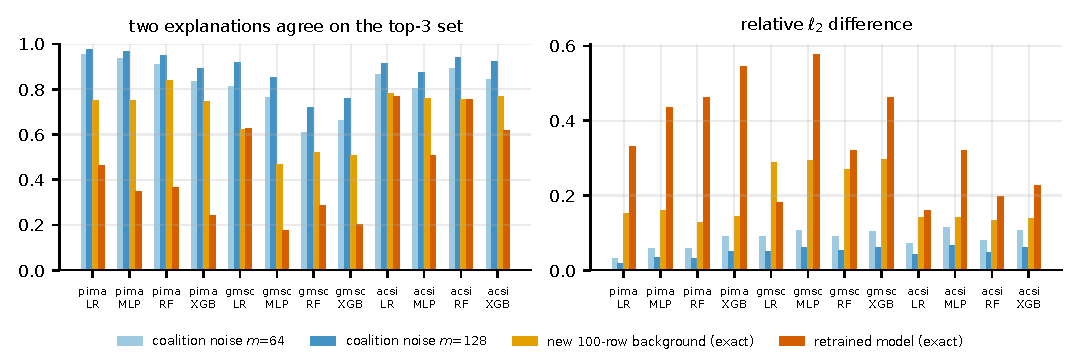
\includegraphics[width=\textwidth]{figs/fig_standards.pdf}
\caption{Agreement between two explanations of the same instance that differ in one source only. Coalition-sampling noise of a single run (Kernel SHAP, $m{=}64$, $128$) vs.\ two exact explanations from independently drawn 100-row backgrounds or from two bootstrap-retrained models ($K{=}8$ models; AUC range at most 0.04 per cell). Datasets with $d\le10$, 50 instances per cell. Left: same top-3 set. Right: relative $\ell_2$ difference.}\label{fig:std}
\end{figure}
Is estimator noise large compared to other things that change an explanation? Fig.~\ref{fig:std} (Appendix Table~\ref{tab:std}) compares the pairwise agreement of two single runs with that of two \emph{exact} explanations that differ only by (a) the 100 background rows, redrawn from a reference sample of 500--1000 rows, or (b) retraining on a bootstrap resample of the training set with a new seed (the test AUC of the 8 models per cell spans at most 0.04). At $m=128$ two runs agree on the top-3 set in 81--95\% of cases (dataset means over the 4 models), whereas two backgrounds agree in 53--77\% and two retrained models in 32--66\%; for relative $\ell_2$ differences the order is the same (0.03--0.06 vs.\ 0.14--0.29 vs.\ 0.23--0.44). For $d\le10$ there is thus no case for spending compute on more repeated runs while the background and the model remain as variable as they are; conversely, redrawing a 100-row background between runs adds far more variation than coalition sampling. Fixed-budget view (Fig.~\ref{fig:bg}): with total budget $N=m\cdot b$ model calls, reliability against the 1000-row reference explanation is nearly flat in $m$ once $m\ge64$ and increases with $b$ (ACSIncome, $N=2\cdot10^4$--$10^5$: top-3 set correct 0.66--0.68 at $b{=}25$, 0.82--0.83 at $b{=}100$, 0.86--0.89 at $b{=}250$; GMSC: 0.41--0.43, 0.64--0.65, 0.78--0.80); the best use of a fixed budget is to enlarge the background and keep $m$ at a few hundred. (Because the reference itself is a finite sample, the advantage of large $b$ is partly an overlap effect; the monotone trend, not the absolute level, is the evidence.)
\begin{figure}[t]
\centering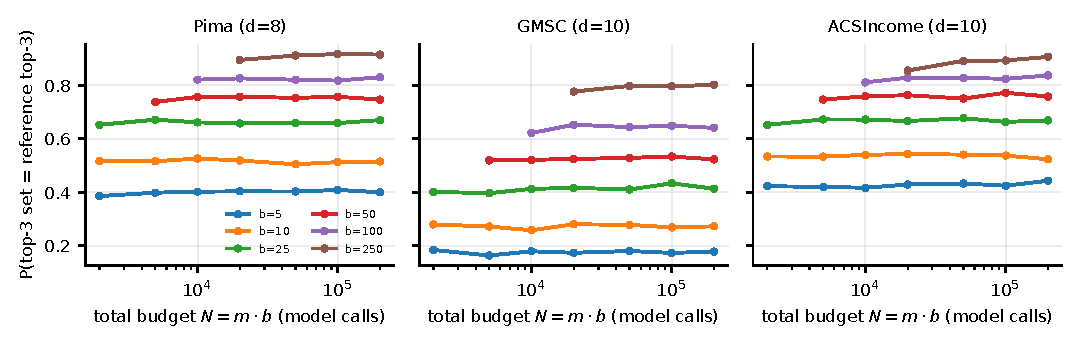
\includegraphics[width=\textwidth]{figs/fig_background.pdf}
\caption{Fixed model-call budget $N=m\,b$ split between coalitions $m$ and background rows $b$ (Kernel SHAP, fresh random background per run, 4 models, 50 instances, 20 runs). Only $m\ge64$ is shown; where $2^d-2<N/b$ all coalitions are enumerated.}\label{fig:bg}
\end{figure}

\subsection{A high-dimensional stress test}\label{sec:highd}
To probe $d$ far beyond what can be tabulated we use UCI Arrhythmia \citep{arrhythmia} ($d{=}262$ non-constant features, 316 training rows, XGBoost, test AUC 0.870, log-odds output), where the exact interventional TreeSHAP values with the same 100-row background are the ground truth (additivity error $\le10^{-6}$), 16 instances, 20 runs per setting, real model calls. Table~\ref{tab:highd} shows that, for this model, our Kernel SHAP is accurate at the library budget $m{\approx}2d{+}2048$: top-1 always correct and top-3 correct in 99\% (95\% CI over instances 0.97--1.00) at $m=2048$ (the library with \texttt{l1\_reg=False}: 95\% [0.86, 1.00] at 2572 coalitions, so the two overlap within the small-sample noise) ($m<2d$ is unusable: top-3 correct in only 73\% at $m=512$). This is not a general statement about high dimensions: for this model the 10 largest attributions carry on average 74\% of $\|\phi\|_2^2$ (minimum 49\%), so most players are nearly irrelevant. The library default, however, collapses: median relative error 0.62, top-1 correct 65\%, top-3 41\%, because LARS keeps 10 of 262 features.
\begin{table}[t]
\centering\scriptsize
\begin{tabular}{llccc}
\toprule
Estimator & $m$ & median rel.\ $\ell_2$ err. & top-1 correct & top-3 set correct\\
\midrule
Kernel SHAP (ours, no L1) & 1024 & 0.051 & 0.997 [0.99,1.00] & 0.962 [0.90,1.00]\\
Kernel SHAP (ours, no L1) & 2048 & 0.031 & 1.000 [1.00,1.00] & 0.991 [0.97,1.00]\\
Kernel SHAP (ours, no L1) & 8192 & 0.013 & 1.000 [1.00,1.00] & 0.988 [0.97,1.00]\\
Leverage SHAP (ours) & 1024 & 0.037 & 1.000 [1.00,1.00] & 0.947 [0.88,1.00]\\
Leverage SHAP (ours) & 2048 & 0.020 & 0.997 [0.99,1.00] & 0.963 [0.91,1.00]\\
Leverage SHAP (ours) & 8192 & 0.009 & 1.000 [1.00,1.00] & 0.975 [0.93,1.00]\\
shap.KernelExplainer, l1\_reg=False & 2572 & 0.021 & 1.000 [1.00,1.00] & 0.950 [0.86,1.00]\\
shap.KernelExplainer, default & 2572 & 0.623 & 0.650 [0.42,0.86] & 0.412 [0.21,0.64]\\
\bottomrule
\end{tabular}
\caption{Arrhythmia ($d{=}262$): comparison with exact TreeSHAP; 16 instances, mean over instances with 95\% bootstrap CI.}\label{tab:highd}
\end{table}

\section{Discussion and limitations}
\textbf{Verdict.} The answer to ``can a single run be taken as the basis of the prediction?'' is conditional. For the \emph{top-1} claim, yes at almost any budget $\ge$256 on our data (98\%+ correct). For the \emph{top-3 set}, yes at $m\approx2048$ for most instances (98.4\% of runs; 94\% of instances meet a 90\% repeatability bar) but not at $m\le256$ for a fifth of instances, and not for the near-tie instances (about one in five at $d\ge16$) at any budget---there the question is ill-posed rather than under-sampled. For complete enumeration ($d\lesssim10$) there is no noise to worry about. A single run is also adequate in a more relative sense: coalition noise is much smaller than the changes due to retraining or the background draw. What fails is not the single run itself but unverified single runs: a free within-run $z$ statistic identifies the runs that cannot be trusted, and the \texttt{shap} defaults may bias the result in a way no repetition would reveal.

\textbf{Limitations.} (1) \emph{Scale:} $d\le20$ for tabulated ground truth and one stress test at $d{=}262$ with trees; non-additive high-dimensional games are not covered, so the budget requirements we measure should not be extrapolated to e.g.\ $d\ge50$ with strong interactions. (2) \emph{Value function:} interventional with a fixed 100-row background, probability output (log-odds for the stress test); conditional/observational variants \citep{chen2020} and other outputs were not studied. (3) \emph{Models and instances:} four standard model families, one trained model per cell (plus a replicate and the retraining experiment), 24 instances for $d{=}20$; CIs reflect instance sampling, not model-training randomness; the replicate (Appendix~\ref{app:rep}) shows cell-level differences of up to 16 points in top-3 correctness, so absolute levels are model-specific, and the German results are the least precise. Tree models have an exact algorithm \citep{lundberg2020} and our findings concern model-agnostic use. (4) \emph{Criteria:} the 0.9 level, top-3 and exact-set claims are conventions; other claims (e.g.\ values within 10\%, sign) give different budgets. (5) \emph{Estimators:} our Kernel SHAP is a port of the library's sampling logic, validated against the library but not identical (duplicate handling); Leverage SHAP is our re-implementation (without-replacement schemes and the authors' tuning are not included), so its null result is not a statement about the original. (6) The background experiment uses a finite reference sample; its absolute levels are optimistic for large $b$. (7) The certificate's SE assumes iid coalition draws and underestimates at $d{=}20$ and $m\le128$; we evaluated one certificate form, and the calibration at tail error rates has wide intervals.

\textbf{Conclusion.} Single-run SHAP is reliable for coarse claims at moderate budgets, unreliable for fine rankings at low budgets or at near-ties, and its largest practical risks are the background and library defaults rather than coalition noise. We recommend reporting the budget, using enumeration for $d\lesssim10$, using the within-run $z$ to flag unresolvable rankings, and checking default settings such as \texttt{l1\_reg}.

\bibliographystyle{plainnat}
\bibliography{refs}

\appendix
\section{Estimator details}\label{app:est}
Let $k(S)\propto 1/(\binom{d}{|S|}|S|(d-|S|))$ be the Shapley kernel. \emph{Kernel SHAP.} Size classes $s=1..\lceil (d-1)/2\rceil$ stand for sizes $s$ and $d-s$ (paired). Starting from the cheapest class, a class is enumerated completely (with complements) if its share of the remaining budget covers it; otherwise sizes are drawn with probability proportional to the kernel mass of the remaining classes, a random coalition of that size is drawn and its complement added; a repeated coalition increments the weight of the existing row; sampling stops when $m$ rows exist. Sampled rows jointly receive the kernel mass left after enumeration, in proportion to counts; the regression with the sum-to-effect constraint is solved by elimination of the last player (as in \texttt{shap}). \emph{Leverage SHAP}: identical, but the size class is drawn uniformly over the remaining classes and each draw contributes weight $k(S)\binom{d}{|S|}/(\pi_s N)$ ($\pi_s$ the class probability, $N$ the number of draws). The leverage scores of the rows of the constrained design $\sqrt{k(S)}Z_S$ equal $1/\binom{d}{|S|}$ (checked numerically for $d=7$). \emph{Permutation SHAP}: $\lfloor m/(2(d-1))\rfloor$ forward/reverse permutation pairs. Unbiasedness and SE calibration were checked on random games with $d=10,20$ (code \texttt{test\_est.py}).

\section{Setup details}\label{app:setup}
Models: LR (C=1); MLP $64{-}64$ ReLU, Adam, $\alpha=10^{-3}$ with early stopping for $n_{\rm train}\ge5000$, $\alpha=1$, 50 epochs without early stopping for smaller data (chosen from 5 splits of German/Pima to avoid the overfitting seen with early stopping on 10\% validation); RF 100 trees (50 if $n_{\rm train}<1000$), min leaf 5 (20 if $n\ge5000$), $\sqrt d$ features; XGBoost 150 trees, depth 4, learning rate 0.1, subsample 0.8, column sample 0.8. Preprocessing is fit on the training split: median imputation; quantile-normal transform of numeric features and one-hot of categoricals for LR/MLP, ordinal codes for trees; high-cardinality ACS features (OCCP, POBP) use smoothed target means. Background rows: $b_{\rm ref}$ random training rows; the main experiment uses the first 100. German credit contains protected attributes (sex, age); we use it only as a benchmark. Pima zeros are not treated as missing. Seeds: instance sampling 123, background 1, split 0 (replicate: 1), per-run seeds from a hash of (dataset, model, instance, $m$, estimator, run).

\section{Further results}\label{app:more}
\begin{table}[h]
\centering\scriptsize\setlength{\tabcolsep}{3pt}
\begin{tabular}{llcccccc}
\toprule
 & & \multicolumn{3}{c}{$m=256$} & \multicolumn{3}{c}{$m=2048$}\\
\cmidrule(lr){3-5}\cmidrule(lr){6-8}
Dataset & Model & top-1 & top-3 set & \% inst.\ $\ge$0.9 & top-1 & top-3 set & \% inst.\ $\ge$0.9\\
\midrule
Pima (d=8) & LR & enum. & enum. & enum. & enum. & enum. & enum.\\
Pima (d=8) & MLP & enum. & enum. & enum. & enum. & enum. & enum.\\
Pima (d=8) & RF & enum. & enum. & enum. & enum. & enum. & enum.\\
Pima (d=8) & XGB & enum. & enum. & enum. & enum. & enum. & enum.\\
GMSC (d=10) & LR & 99.7 & 98.3 & 95.0 & enum. & enum. & enum.\\
GMSC (d=10) & MLP & 99.1 & 93.4 & 77.0 & enum. & enum. & enum.\\
GMSC (d=10) & RF & 99.6 & 86.1 & 56.0 & enum. & enum. & enum.\\
GMSC (d=10) & XGB & 98.7 & 88.3 & 63.0 & enum. & enum. & enum.\\
ACSIncome (d=10) & LR & 99.0 & 96.5 & 87.0 & enum. & enum. & enum.\\
ACSIncome (d=10) & MLP & 98.1 & 93.3 & 82.0 & enum. & enum. & enum.\\
ACSIncome (d=10) & RF & 98.6 & 97.2 & 92.0 & enum. & enum. & enum.\\
ACSIncome (d=10) & XGB & 98.2 & 96.8 & 90.0 & enum. & enum. & enum.\\
ACSEmployment (d=16) & LR & 99.9 & 97.0 & 93.3 & 100.0 & 99.3 & 96.7\\
ACSEmployment (d=16) & MLP & 96.1 & 92.5 & 78.3 & 98.1 & 98.0 & 93.3\\
ACSEmployment (d=16) & RF & 96.9 & 97.6 & 91.7 & 98.6 & 99.7 & 98.3\\
ACSEmployment (d=16) & XGB & 99.3 & 91.5 & 75.0 & 99.8 & 97.9 & 95.0\\
German (d=20) & LR & 100.0 & 95.4 & 87.5 & 100.0 & 98.4 & 95.8\\
German (d=20) & MLP & 98.3 & 85.8 & 58.3 & 100.0 & 96.7 & 87.5\\
German (d=20) & RF & 98.6 & 92.3 & 75.0 & 99.9 & 98.6 & 91.7\\
German (d=20) & XGB & 96.0 & 92.5 & 75.0 & 99.0 & 99.0 & 91.7\\
\bottomrule
\end{tabular}
\caption{Kernel SHAP single-run reliability per dataset and model (\%): top-1, top-3 set correct (means over runs and instances) and fraction of instances for which the top-3 claim is correct in $\ge$90\% of runs. ``enum.'': $m\ge2^d-2$, complete enumeration (exact). CIs are in \texttt{results/summary} (code \texttt{analyze\_figs.py}).}\label{tab:rel}
\end{table}
\begin{table}[h]
\centering\scriptsize\setlength{\tabcolsep}{3pt}
\begin{tabular}{llcccc}
\toprule
Dataset & Source of variation & top-1 agree & top-3 set agree & RBO & rel.\ $\ell_2$ diff.\\
\midrule
Pima & coalition sampling, $m{=}64$ & 0.969 & 0.908 & 0.980 & 0.060\\
Pima & coalition sampling, $m{=}128$ & 0.981 & 0.946 & 0.988 & 0.034\\
Pima & new 25-row background (exact) & 0.827 & 0.558 & 0.927 & 0.317\\
Pima & new 100-row background (exact) & 0.919 & 0.770 & 0.962 & 0.146\\
Pima & retrained model (exact) & 0.743 & 0.356 & 0.888 & 0.444\\
\midrule
GMSC & coalition sampling, $m{=}64$ & 0.966 & 0.711 & 0.960 & 0.098\\
GMSC & coalition sampling, $m{=}128$ & 0.980 & 0.811 & 0.975 & 0.057\\
GMSC & new 25-row background (exact) & 0.655 & 0.302 & 0.851 & 0.603\\
GMSC & new 100-row background (exact) & 0.811 & 0.530 & 0.919 & 0.287\\
GMSC & retrained model (exact) & 0.817 & 0.323 & 0.881 & 0.385\\
\midrule
ACSIncome & coalition sampling, $m{=}64$ & 0.946 & 0.851 & 0.964 & 0.093\\
ACSIncome & coalition sampling, $m{=}128$ & 0.969 & 0.913 & 0.978 & 0.054\\
ACSIncome & new 25-row background (exact) & 0.838 & 0.565 & 0.921 & 0.291\\
ACSIncome & new 100-row background (exact) & 0.922 & 0.766 & 0.960 & 0.139\\
ACSIncome & retrained model (exact) & 0.849 & 0.662 & 0.932 & 0.226\\
\bottomrule
\end{tabular}
\caption{Pairwise agreement of two explanations differing in one source of variation (dataset means over 4 models, 50 instances; $d\le10$). Coalition sampling: two independent single Kernel SHAP runs.}\label{tab:std}
\end{table}
\begin{table}[h]
\centering\scriptsize\setlength{\tabcolsep}{3pt}
\begin{tabular}{llrcccc}
\toprule
Dataset & Variant & $m$ & lib: med.\ rel.\ err. & sim: med.\ rel.\ err. & lib: top-3 ok & sim: top-3 ok\\
\midrule
Pima & Kernel, l1\_reg=False & 64 & 0.072 & 0.067 & 0.806 & 0.843\\
Pima & Permutation & 64 & 0.067 & 0.054 & 0.812 & 0.805\\
\midrule
ACSIncome & Kernel, l1\_reg=False & 64 & 0.066 & 0.061 & 0.844 & 0.862\\
ACSIncome & Kernel, l1\_reg=False & 256 & 0.022 & 0.021 & 0.969 & 0.959\\
ACSIncome & Permutation & 64 & 0.065 & 0.056 & 0.869 & 0.850\\
ACSIncome & Permutation & 256 & 0.024 & 0.025 & 0.894 & 0.900\\
\midrule
ACSEmployment & Kernel, l1\_reg=False & 64 & 0.124 & 0.122 & 0.812 & 0.847\\
ACSEmployment & Kernel, l1\_reg=False & 256 & 0.042 & 0.041 & 0.950 & 0.966\\
ACSEmployment & Kernel, l1\_reg=False & 2080 & 0.012 & 0.011 & 1.000 & 0.998\\
ACSEmployment & Permutation & 64 & 0.090 & 0.053 & 0.869 & 0.926\\
ACSEmployment & Permutation & 256 & 0.030 & 0.026 & 0.962 & 0.955\\
ACSEmployment & Kernel, default l1\_reg & 256 & 0.049 & 0.041 & 0.962 & 0.966\\
ACSEmployment & Kernel, default l1\_reg & 2080 & 0.031 & 0.011 & 1.000 & 0.998\\
\midrule
German & Kernel, l1\_reg=False & 64 & 0.195 & 0.217 & 0.806 & 0.770\\
German & Kernel, l1\_reg=False & 256 & 0.061 & 0.067 & 0.956 & 0.963\\
German & Kernel, l1\_reg=False & 2088 & 0.018 & 0.020 & 1.000 & 1.000\\
German & Permutation & 64 & 0.154 & 0.168 & 0.781 & 0.757\\
German & Permutation & 256 & 0.073 & 0.066 & 0.925 & 0.939\\
German & Kernel, default l1\_reg & 256 & 0.223 & 0.067 & 0.875 & 0.963\\
German & Kernel, default l1\_reg & 2088 & 0.210 & 0.020 & 0.988 & 1.000\\
\bottomrule
\end{tabular}
\caption{Real \texttt{shap} 0.51.0 library (XGBoost, 8 instances $\times$ 20 repeats) vs.\ the table-oracle estimator on the same instances (``sim''; for $m$=``auto'' the library uses $2d{+}2048$, sim $m{=}2048$). Median relative $\ell_2$ error and top-3 set correctness.}\label{tab:lib}
\end{table}
\begin{figure}[h]
\centering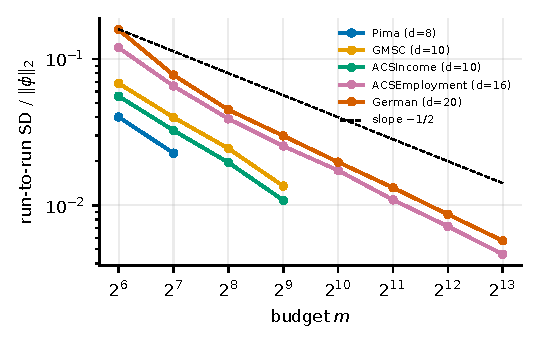
\includegraphics[width=0.55\textwidth]{figs/fig_sd.pdf}
\caption{Run-to-run SD of the attribution vector relative to $\|\phi\|_2$ (median over instances; Kernel SHAP), by dataset; the dashed line has slope $-1/2$ for reference.}\label{fig:sd}
\end{figure}

\section{Replicate with a second split and model seed}\label{app:rep}
To see how much a different trained model changes the picture, we repeated the main experiment for the $d\le10$ datasets with a different split and model seed (seed 1; all else equal; 100 instances per cell). Table~\ref{tab:rep} shows top-3 correctness at two budgets. The mean absolute difference between replicates over the 12 cells is 3.8 points at $m{=}128$ (3.2 for the 8 cells that are not fully enumerated at $m{=}256$), but individual cells differ by up to 15.8 points (GMSC random forest: 79.0\% vs.\ 94.8\% at $m{=}128$; XGBoost 82.7\% vs.\ 94.4\%). The cause is the instance margin, not the noise: the median run-to-run SD of the attribution (relative to $\|\phi\|_2$) is 0.036 vs.\ 0.034 for GMSC-RF, but 54\% of the explained instances of the first model have an exact gap $a_{(3)}-a_{(4)}<0.02\|\phi\|_2$ versus 13\% for the replicate. So absolute reliability levels in \S4 are model-specific, which our instance-level intervals do not cover; the mechanism of \S\ref{sec:mech} (reliability is set by gap-to-noise) is unchanged.
\begin{table}[h]
\centering\scriptsize\setlength{\tabcolsep}{3pt}
\begin{tabular}{llcccccc}
\toprule
Dataset & Model & \multicolumn{3}{c}{top-3 set correct (\%), $m{=}128$} & \multicolumn{3}{c}{top-3 set correct (\%), $m{=}256$}\\
\cmidrule(lr){3-5}\cmidrule(lr){6-8}
 & & main & replicate & AUC (m/r) & main & replicate & AUC (m/r)\\
\midrule
pima & LR & 98.4 & 97.6 & 0.867/0.814 & enum. & enum. & 0.867/0.814\\
pima & MLP & 97.9 & 94.1 & 0.869/0.794 & enum. & enum. & 0.869/0.794\\
pima & RF & 96.3 & 96.3 & 0.847/0.809 & enum. & enum. & 0.847/0.809\\
pima & XGB & 91.5 & 94.4 & 0.834/0.790 & enum. & enum. & 0.834/0.790\\
gmsc & LR & 95.1 & 95.8 & 0.853/0.853 & 98.3 & 97.0 & 0.853/0.853\\
gmsc & MLP & 89.3 & 93.7 & 0.864/0.861 & 93.4 & 95.0 & 0.864/0.861\\
gmsc & RF & 79.0 & 94.8 & 0.865/0.869 & 86.1 & 96.5 & 0.865/0.869\\
gmsc & XGB & 82.7 & 94.4 & 0.866/0.872 & 88.3 & 96.8 & 0.866/0.872\\
acsincome & LR & 94.1 & 95.7 & 0.889/0.889 & 96.5 & 97.4 & 0.889/0.889\\
acsincome & MLP & 90.7 & 92.1 & 0.899/0.897 & 93.3 & 95.0 & 0.899/0.897\\
acsincome & RF & 95.6 & 93.8 & 0.898/0.897 & 97.2 & 96.3 & 0.898/0.897\\
acsincome & XGB & 94.4 & 94.0 & 0.902/0.901 & 96.8 & 97.1 & 0.902/0.901\\
\bottomrule
\end{tabular}
\caption{Main models (seed 0) vs.\ replicate models (split/model seed 1), Kernel SHAP, $d\le10$ datasets; AUC of both models given. ``enum.'': complete enumeration.}\label{tab:rep}
\end{table}

\section{Reproducibility and compute}
Code, exact commands, versions and the mapping from tables/figures to scripts are in \texttt{README.md}; all numbers in this paper are produced by the scripts in \texttt{code/}. Total compute was about 10 CPU-hours for the final pipeline (about 3 more for aborted and exploratory runs; estimated as wall-clock times the 4-core quota; main experiment 4.9, background/retraining/pairing 1.0, library validation 0.7, stress test 1.8, replicate 1.1) CPU-hours on a machine whose cgroup quota is 4 cores. No dataset or result in this paper is synthetic; tabulated games are exact computations on the trained models.

\section*{NeurIPS Paper Checklist}




\begin{enumerate}

\item {\bf Claims}
    \item[] Question: Do the main claims made in the abstract and introduction accurately reflect the paper's contributions and scope?
    \item[] Answer: \answerYes{} % Replace by \answerYes{}, \answerNo{}, or \answerNA{}.
    \item[] Justification: Abstract and introduction state the claims (conditional reliability, certificate, yardsticks, library defaults) with the evidence in Sec.~4 and the scope ($d\le20$ tabulated, one $d{=}262$ stress test) in Sec.~5.
    \item[] Guidelines:
    \begin{itemize}
        \item The answer \answerNA{} means that the abstract and introduction do not include the claims made in the paper.
        \item The abstract and/or introduction should clearly state the claims made, including the contributions made in the paper and important assumptions and limitations. A \answerNo{} or \answerNA{} answer to this question will not be perceived well by the reviewers. 
        \item The claims made should match theoretical and experimental results, and reflect how much the results can be expected to generalize to other settings. 
        \item It is fine to include aspirational goals as motivation as long as it is clear that these goals are not attained by the paper. 
    \end{itemize}

\item {\bf Limitations}
    \item[] Question: Does the paper discuss the limitations of the work performed by the authors?
    \item[] Answer: \answerYes{} % Replace by \answerYes{}, \answerNo{}, or \answerNA{}.
    \item[] Justification: Sec.~5 (limitations paragraph) lists scale, value function, models/instances, criteria, estimator re-implementations, finite reference sample and certificate assumptions.
    \item[] Guidelines:
    \begin{itemize}
        \item The answer \answerNA{} means that the paper has no limitation while the answer \answerNo{} means that the paper has limitations, but those are not discussed in the paper. 
        \item The authors are encouraged to create a separate ``Limitations'' section in their paper.
        \item The paper should point out any strong assumptions and how robust the results are to violations of these assumptions (e.g., independence assumptions, noiseless settings, model well-specification, asymptotic approximations only holding locally). The authors should reflect on how these assumptions might be violated in practice and what the implications would be.
        \item The authors should reflect on the scope of the claims made, e.g., if the approach was only tested on a few datasets or with a few runs. In general, empirical results often depend on implicit assumptions, which should be articulated.
        \item The authors should reflect on the factors that influence the performance of the approach. For example, a facial recognition algorithm may perform poorly when image resolution is low or images are taken in low lighting. Or a speech-to-text system might not be used reliably to provide closed captions for online lectures because it fails to handle technical jargon.
        \item The authors should discuss the computational efficiency of the proposed algorithms and how they scale with dataset size.
        \item If applicable, the authors should discuss possible limitations of their approach to address problems of privacy and fairness.
        \item While the authors might fear that complete honesty about limitations might be used by reviewers as grounds for rejection, a worse outcome might be that reviewers discover limitations that aren't acknowledged in the paper. The authors should use their best judgment and recognize that individual actions in favor of transparency play an important role in developing norms that preserve the integrity of the community. Reviewers will be specifically instructed to not penalize honesty concerning limitations.
    \end{itemize}

\item {\bf Theory assumptions and proofs}
    \item[] Question: For each theoretical result, does the paper provide the full set of assumptions and a complete (and correct) proof?
    \item[] Answer: \answerNA{} % Replace by \answerYes{}, \answerNo{}, or \answerNA{}.
    \item[] Justification: No theoretical results; the Gaussian approximation $\Phi(z)$ is used only as an empirical reference curve.
    \item[] Guidelines:
    \begin{itemize}
        \item The answer \answerNA{} means that the paper does not include theoretical results. 
        \item All the theorems, formulas, and proofs in the paper should be numbered and cross-referenced.
        \item All assumptions should be clearly stated or referenced in the statement of any theorems.
        \item The proofs can either appear in the main paper or the supplemental material, but if they appear in the supplemental material, the authors are encouraged to provide a short proof sketch to provide intuition. 
        \item Inversely, any informal proof provided in the core of the paper should be complemented by formal proofs provided in appendix or supplemental material.
        \item Theorems and Lemmas that the proof relies upon should be properly referenced. 
    \end{itemize}

    \item {\bf Experimental result reproducibility}
    \item[] Question: Does the paper fully disclose all the information needed to reproduce the main experimental results of the paper to the extent that it affects the main claims and/or conclusions of the paper (regardless of whether the code and data are provided or not)?
    \item[] Answer: \answerYes{} % Replace by \answerYes{}, \answerNo{}, or \answerNA{}.
    \item[] Justification: Sec.~3 and Appendices A--B, plus the README, give data versions, preprocessing, models, hyper-parameters, estimators, budgets, seeds, and the commands that produce each table and figure.
    \item[] Guidelines:
    \begin{itemize}
        \item The answer \answerNA{} means that the paper does not include experiments.
        \item If the paper includes experiments, a \answerNo{} answer to this question will not be perceived well by the reviewers: Making the paper reproducible is important, regardless of whether the code and data are provided or not.
        \item If the contribution is a dataset and\slash or model, the authors should describe the steps taken to make their results reproducible or verifiable. 
        \item Depending on the contribution, reproducibility can be accomplished in various ways. For example, if the contribution is a novel architecture, describing the architecture fully might suffice, or if the contribution is a specific model and empirical evaluation, it may be necessary to either make it possible for others to replicate the model with the same dataset, or provide access to the model. In general. releasing code and data is often one good way to accomplish this, but reproducibility can also be provided via detailed instructions for how to replicate the results, access to a hosted model (e.g., in the case of a large language model), releasing of a model checkpoint, or other means that are appropriate to the research performed.
        \item While NeurIPS does not require releasing code, the conference does require all submissions to provide some reasonable avenue for reproducibility, which may depend on the nature of the contribution. For example
        \begin{enumerate}
            \item If the contribution is primarily a new algorithm, the paper should make it clear how to reproduce that algorithm.
            \item If the contribution is primarily a new model architecture, the paper should describe the architecture clearly and fully.
            \item If the contribution is a new model (e.g., a large language model), then there should either be a way to access this model for reproducing the results or a way to reproduce the model (e.g., with an open-source dataset or instructions for how to construct the dataset).
            \item We recognize that reproducibility may be tricky in some cases, in which case authors are welcome to describe the particular way they provide for reproducibility. In the case of closed-source models, it may be that access to the model is limited in some way (e.g., to registered users), but it should be possible for other researchers to have some path to reproducing or verifying the results.
        \end{enumerate}
    \end{itemize}


\item {\bf Open access to data and code}
    \item[] Question: Does the paper provide open access to the data and code, with sufficient instructions to faithfully reproduce the main experimental results, as described in supplemental material?
    \item[] Answer: \answerYes{} % Replace by \answerYes{}, \answerNo{}, or \answerNA{}.
    \item[] Justification: All code, the README with commands, environment versions and expected run times are included in the supplementary material; datasets are public (UCI, OpenML, ACS PUMS via folktables) and downloaded by \texttt{get\_data.py}.
    \item[] Guidelines:
    \begin{itemize}
        \item The answer \answerNA{} means that paper does not include experiments requiring code.
        \item Please see the NeurIPS code and data submission guidelines (\url{https://neurips.cc/public/guides/CodeSubmissionPolicy}) for more details.
        \item While we encourage the release of code and data, we understand that this might not be possible, so \answerNo{} is an acceptable answer. Papers cannot be rejected simply for not including code, unless this is central to the contribution (e.g., for a new open-source benchmark).
        \item The instructions should contain the exact command and environment needed to run to reproduce the results. See the NeurIPS code and data submission guidelines (\url{https://neurips.cc/public/guides/CodeSubmissionPolicy}) for more details.
        \item The authors should provide instructions on data access and preparation, including how to access the raw data, preprocessed data, intermediate data, and generated data, etc.
        \item The authors should provide scripts to reproduce all experimental results for the new proposed method and baselines. If only a subset of experiments are reproducible, they should state which ones are omitted from the script and why.
        \item At submission time, to preserve anonymity, the authors should release anonymized versions (if applicable).
        \item Providing as much information as possible in supplemental material (appended to the paper) is recommended, but including URLs to data and code is permitted.
    \end{itemize}


\item {\bf Experimental setting/details}
    \item[] Question: Does the paper specify all the training and test details (e.g., data splits, hyperparameters, how they were chosen, type of optimizer) necessary to understand the results?
    \item[] Answer: \answerYes{} % Replace by \answerYes{}, \answerNo{}, or \answerNA{}.
    \item[] Justification: Sec.~3 and Appendix B: splits (stratified 70/30), hyper-parameters (fixed a priori; MLP regularisation chosen on 5 splits of the small datasets, see Appendix B), instances, backgrounds, seeds.
    \item[] Guidelines:
    \begin{itemize}
        \item The answer \answerNA{} means that the paper does not include experiments.
        \item The experimental setting should be presented in the core of the paper to a level of detail that is necessary to appreciate the results and make sense of them.
        \item The full details can be provided either with the code, in appendix, or as supplemental material.
    \end{itemize}

\item {\bf Experiment statistical significance}
    \item[] Question: Does the paper report error bars suitably and correctly defined or other appropriate information about the statistical significance of the experiments?
    \item[] Answer: \answerYes{} % Replace by \answerYes{}, \answerNo{}, or \answerNA{}.
    \item[] Justification: 95\% cluster-bootstrap intervals over instances (resampling within dataset$\times$model cells) are reported for headline numbers; Sec.~3 states what they do and do not cover (not model-training randomness).
    \item[] Guidelines:
    \begin{itemize}
        \item The answer \answerNA{} means that the paper does not include experiments.
        \item The authors should answer \answerYes{} if the results are accompanied by error bars, confidence intervals, or statistical significance tests, at least for the experiments that support the main claims of the paper.
        \item The factors of variability that the error bars are capturing should be clearly stated (for example, train/test split, initialization, random drawing of some parameter, or overall run with given experimental conditions).
        \item The method for calculating the error bars should be explained (closed form formula, call to a library function, bootstrap, etc.)
        \item The assumptions made should be given (e.g., Normally distributed errors).
        \item It should be clear whether the error bar is the standard deviation or the standard error of the mean.
        \item It is OK to report 1-sigma error bars, but one should state it. The authors should preferably report a 2-sigma error bar than state that they have a 96\% CI, if the hypothesis of Normality of errors is not verified.
        \item For asymmetric distributions, the authors should be careful not to show in tables or figures symmetric error bars that would yield results that are out of range (e.g., negative error rates).
        \item If error bars are reported in tables or plots, the authors should explain in the text how they were calculated and reference the corresponding figures or tables in the text.
    \end{itemize}

\item {\bf Experiments compute resources}
    \item[] Question: For each experiment, does the paper provide sufficient information on the computer resources (type of compute workers, memory, time of execution) needed to reproduce the experiments?
    \item[] Answer: \answerYes{} % Replace by \answerYes{}, \answerNo{}, or \answerNA{}.
    \item[] Justification: Appendix E (compute) gives CPU-hours, the 4-core quota and the memory footprint; the README lists wall-clock per experiment.
    \item[] Guidelines:
    \begin{itemize}
        \item The answer \answerNA{} means that the paper does not include experiments.
        \item The paper should indicate the type of compute workers CPU or GPU, internal cluster, or cloud provider, including relevant memory and storage.
        \item The paper should provide the amount of compute required for each of the individual experimental runs as well as estimate the total compute. 
        \item The paper should disclose whether the full research project required more compute than the experiments reported in the paper (e.g., preliminary or failed experiments that didn't make it into the paper). 
    \end{itemize}
    
\item {\bf Code of ethics}
    \item[] Question: Does the research conducted in the paper conform, in every respect, with the NeurIPS Code of Ethics \url{https://neurips.cc/public/EthicsGuidelines}?
    \item[] Answer: \answerYes{} % Replace by \answerYes{}, \answerNo{}, or \answerNA{}.
    \item[] Justification: The work uses public benchmark data (German Credit contains protected attributes and is used only as a benchmark), involves no human subjects, and does not deviate from the Code of Ethics.
    \item[] Guidelines:
    \begin{itemize}
        \item The answer \answerNA{} means that the authors have not reviewed the NeurIPS Code of Ethics.
        \item If the authors answer \answerNo, they should explain the special circumstances that require a deviation from the Code of Ethics.
        \item The authors should make sure to preserve anonymity (e.g., if there is a special consideration due to laws or regulations in their jurisdiction).
    \end{itemize}


\item {\bf Broader impacts}
    \item[] Question: Does the paper discuss both potential positive societal impacts and negative societal impacts of the work performed?
    \item[] Answer: \answerNA{} % Replace by \answerYes{}, \answerNo{}, or \answerNA{}.
    \item[] Justification: Methodological/empirical study of explanation reliability with no direct deployment; the discussion notes that unverified single-run explanations (and library defaults) can mislead decisions in high-stakes settings.
    \item[] Guidelines:
    \begin{itemize}
        \item The answer \answerNA{} means that there is no societal impact of the work performed.
        \item If the authors answer \answerNA{} or \answerNo, they should explain why their work has no societal impact or why the paper does not address societal impact.
        \item Examples of negative societal impacts include potential malicious or unintended uses (e.g., disinformation, generating fake profiles, surveillance), fairness considerations (e.g., deployment of technologies that could make decisions that unfairly impact specific groups), privacy considerations, and security considerations.
        \item The conference expects that many papers will be foundational research and not tied to particular applications, let alone deployments. However, if there is a direct path to any negative applications, the authors should point it out. For example, it is legitimate to point out that an improvement in the quality of generative models could be used to generate Deepfakes for disinformation. On the other hand, it is not needed to point out that a generic algorithm for optimizing neural networks could enable people to train models that generate Deepfakes faster.
        \item The authors should consider possible harms that could arise when the technology is being used as intended and functioning correctly, harms that could arise when the technology is being used as intended but gives incorrect results, and harms following from (intentional or unintentional) misuse of the technology.
        \item If there are negative societal impacts, the authors could also discuss possible mitigation strategies (e.g., gated release of models, providing defenses in addition to attacks, mechanisms for monitoring misuse, mechanisms to monitor how a system learns from feedback over time, improving the efficiency and accessibility of ML).
    \end{itemize}
    
\item {\bf Safeguards}
    \item[] Question: Does the paper describe safeguards that have been put in place for responsible release of data or models that have a high risk for misuse (e.g., pre-trained language models, image generators, or scraped datasets)?
    \item[] Answer: \answerNA{} % Replace by \answerYes{}, \answerNo{}, or \answerNA{}.
    \item[] Justification: No models or data with high misuse risk are released.
    \item[] Guidelines:
    \begin{itemize}
        \item The answer \answerNA{} means that the paper poses no such risks.
        \item Released models that have a high risk for misuse or dual-use should be released with necessary safeguards to allow for controlled use of the model, for example by requiring that users adhere to usage guidelines or restrictions to access the model or implementing safety filters. 
        \item Datasets that have been scraped from the Internet could pose safety risks. The authors should describe how they avoided releasing unsafe images.
        \item We recognize that providing effective safeguards is challenging, and many papers do not require this, but we encourage authors to take this into account and make a best faith effort.
    \end{itemize}

\item {\bf Licenses for existing assets}
    \item[] Question: Are the creators or original owners of assets (e.g., code, data, models), used in the paper, properly credited and are the license and terms of use explicitly mentioned and properly respected?
    \item[] Answer: \answerYes{} % Replace by \answerYes{}, \answerNo{}, or \answerNA{}.
    \item[] Justification: Datasets: UCI (CC BY 4.0: German Credit, Arrhythmia), OpenML (public), ACS PUMS via folktables (MIT code; Census data public; terms not separately stated); libraries (shap, scikit-learn, XGBoost) are cited or named with versions in the README.
    \item[] Guidelines:
    \begin{itemize}
        \item The answer \answerNA{} means that the paper does not use existing assets.
        \item The authors should cite the original paper that produced the code package or dataset.
        \item The authors should state which version of the asset is used and, if possible, include a URL.
        \item The name of the license (e.g., CC-BY 4.0) should be included for each asset.
        \item For scraped data from a particular source (e.g., website), the copyright and terms of service of that source should be provided.
        \item If assets are released, the license, copyright information, and terms of use in the package should be provided. For popular datasets, \url{paperswithcode.com/datasets} has curated licenses for some datasets. Their licensing guide can help determine the license of a dataset.
        \item For existing datasets that are re-packaged, both the original license and the license of the derived asset (if it has changed) should be provided.
        \item If this information is not available online, the authors are encouraged to reach out to the asset's creators.
    \end{itemize}

\item {\bf New assets}
    \item[] Question: Are new assets introduced in the paper well documented and is the documentation provided alongside the assets?
    \item[] Answer: \answerYes{} % Replace by \answerYes{}, \answerNo{}, or \answerNA{}.
    \item[] Justification: The released code and README document the estimators, experiment scripts and the mapping from results to scripts.
    \item[] Guidelines:
    \begin{itemize}
        \item The answer \answerNA{} means that the paper does not release new assets.
        \item Researchers should communicate the details of the dataset\slash code\slash model as part of their submissions via structured templates. This includes details about training, license, limitations, etc. 
        \item The paper should discuss whether and how consent was obtained from people whose asset is used.
        \item At submission time, remember to anonymize your assets (if applicable). You can either create an anonymized URL or include an anonymized zip file.
    \end{itemize}

\item {\bf Crowdsourcing and research with human subjects}
    \item[] Question: For crowdsourcing experiments and research with human subjects, does the paper include the full text of instructions given to participants and screenshots, if applicable, as well as details about compensation (if any)? 
    \item[] Answer: \answerNA{} % Replace by \answerYes{}, \answerNo{}, or \answerNA{}.
    \item[] Justification: No crowdsourcing or human-subject research.
    \item[] Guidelines:
    \begin{itemize}
        \item The answer \answerNA{} means that the paper does not involve crowdsourcing nor research with human subjects.
        \item Including this information in the supplemental material is fine, but if the main contribution of the paper involves human subjects, then as much detail as possible should be included in the main paper. 
        \item According to the NeurIPS Code of Ethics, workers involved in data collection, curation, or other labor should be paid at least the minimum wage in the country of the data collector. 
    \end{itemize}

\item {\bf Institutional review board (IRB) approvals or equivalent for research with human subjects}
    \item[] Question: Does the paper describe potential risks incurred by study participants, whether such risks were disclosed to the subjects, and whether Institutional Review Board (IRB) approvals (or an equivalent approval/review based on the requirements of your country or institution) were obtained?
    \item[] Answer: \answerNA{} % Replace by \answerYes{}, \answerNo{}, or \answerNA{}.
    \item[] Justification: No human subjects, hence no IRB approval is needed.
    \item[] Guidelines:
    \begin{itemize}
        \item The answer \answerNA{} means that the paper does not involve crowdsourcing nor research with human subjects.
        \item Depending on the country in which research is conducted, IRB approval (or equivalent) may be required for any human subjects research. If you obtained IRB approval, you should clearly state this in the paper. 
        \item We recognize that the procedures for this may vary significantly between institutions and locations, and we expect authors to adhere to the NeurIPS Code of Ethics and the guidelines for their institution. 
        \item For initial submissions, do not include any information that would break anonymity (if applicable), such as the institution conducting the review.
    \end{itemize}

\item {\bf Declaration of LLM usage}
    \item[] Question: Does the paper describe the usage of LLMs if it is an important, original, or non-standard component of the core methods in this research? Note that if the LLM is used only for writing, editing, or formatting purposes and does \emph{not} impact the core methodology, scientific rigor, or originality of the research, declaration is not required.
    %this research? 
    \item[] Answer: \answerYes{} % Replace by \answerYes{}, \answerNo{}, or \answerNA{}.
    \item[] Justification: The research (design, code, experiments, analysis and writing) was carried out by an autonomous LLM agent (Claude) running unattended; this is declared here since it is a non-standard component of how the work was produced.
    \item[] Guidelines:
    \begin{itemize}
        \item The answer \answerNA{} means that the core method development in this research does not involve LLMs as any important, original, or non-standard components.
        \item Please refer to our LLM policy in the NeurIPS handbook for what should or should not be described.
    \end{itemize}

\end{enumerate}
\end{document}
